\documentclass{beamer}
\beamertemplatenavigationsymbolsempty
\usecolortheme{beaver}
\setbeamertemplate{blocks}[rounded=true, shadow=true]
\setbeamertemplate{footline}[page number]
%
\usepackage[utf8]{inputenc}
\usepackage[english,russian]{babel}
\usepackage{amssymb,amsfonts,amsmath,mathtext}
\usepackage{subfig}
\usepackage[all]{xy} % xy package for diagrams
\usepackage{array}
\usepackage{multicol}% many columns in slide
\usepackage{hyperref}% urls
\usepackage{hhline}%tables
% Your figures are here:
\graphicspath{ {fig/} {../fig/} }

%----------------------------------------------------------------------------------------------------------
\title{Поиск границ радужки\\ методом круговых проекций}
\author[А.\,А. Баженов]{Баженов Андрей Александрович}
\institute{Московский физико-технический институт}
\date{\footnotesize
\par\smallskip\emph{Курс:} Автоматизация научных исследований\par (практика, В.\,В.~Стрижов)/Группа 821
\par\smallskip\emph{Эксперт:} И.\,А.~Матвеев
\par\smallskip\emph{Консультант:} И.\,А.~Матвеев
\par\bigskip\small 2021}
%----------------------------------------------------------------------------------------------------------
\begin{document}
%----------------------------------------------------------------------------------------------------------
\begin{frame}
\thispagestyle{empty}
\maketitle
\end{frame}
%-----------------------------------------------------------------------------------------------------
%\begin{frame}{Цель исследования}
%\begin{block}{Решается задача}
%\end{block}
%\end{frame}
%-----------------------------------------------------------------------------------------------------
\begin{frame}{Круговые проекции яркости}

\begin{columns}[c]
\column{0.65\textwidth}
		$\vec{x}$~--- точка изображения\\ 
		$\vec{g}(\vec{x})$~--- градиент яркости\\
		$v_U(\vec{x})$~--- индикатор возможности принадлежности границе
		\[
		\Pi_U(r) = \frac{1}{2\pi r} \sum_{r-0.5 \leqslant \| x \| \leqslant r + 0.5} v_U(r)
		\]
\column{0.35\textwidth}
    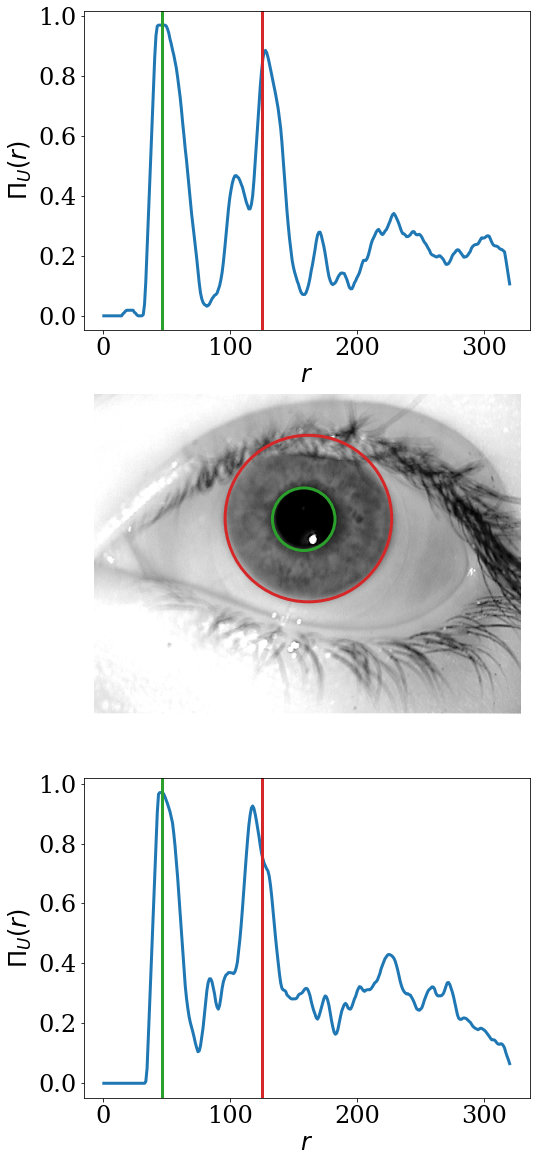
\includegraphics[scale=0.2]{img/eye.png}
\end{columns}

\end{frame}

\end{document}